\documentclass{report}

\usepackage[english]{babel}
\usepackage[utf8]{inputenc}
\usepackage{hyperref}

\usepackage{fancyhdr}
\usepackage {amsmath,amssymb} 
\usepackage{graphicx}
\usepackage{tikz-cd}
\usepackage{amsthm}
\usepackage[all]{xy}
\usepackage[font={footnotesize}]{caption}

\usetikzlibrary{arrows}
\usetikzlibrary{matrix}


\newtheorem*{thm}{Theorem}
\newtheorem*{prop}{Proposition}
\newtheorem*{lemma}{Lemma}
\newtheorem*{coroll}{Corollary}     
\theoremstyle{definition}
\newtheorem*{defi}{Definition}
\newtheorem*{ex}{Example} 
\newtheorem*{exs}{Examples}
\theoremstyle{remark}
\newtheorem*{rk}{Remark}

 \newcommand{\Tt}{\ensuremath{ \{T(t)\}}}
\newcommand{\id}{\ensuremath{\text{I}}}
\newcommand{\la}{\ensuremath{_{\ast}}}
\newcommand{\upa}{\ensuremath{^{\ast}}}

\title{Complex Networks}
\author{{Marco Murtinu, Claudio Peroni}}

\begin{document}
	\maketitle

\section*{Exercise 5.4}

In this exercise we analyze a network representing 50 farmers living along a 50-mile-long stretch of river. Each farmer lives on a portion of land that occupies a 1-mile stretch of the river bank. The farmers all know each other and, after interviewing them, we discovered that each of them is friends with all the neighbors that live at most 20 miles away, and sees as an enemy all the others.\\
To model such situation with a network, the natural choice is an \textit{undirected complete signed network}, where the sign of the edges will represent whether its two endpoints are friends or enemies. We are asked to understand whether such network is \textbf{structurally balanced}.\\
First of all, let us give a look to such network.\\
\begin{figure} [h]
	\centering
	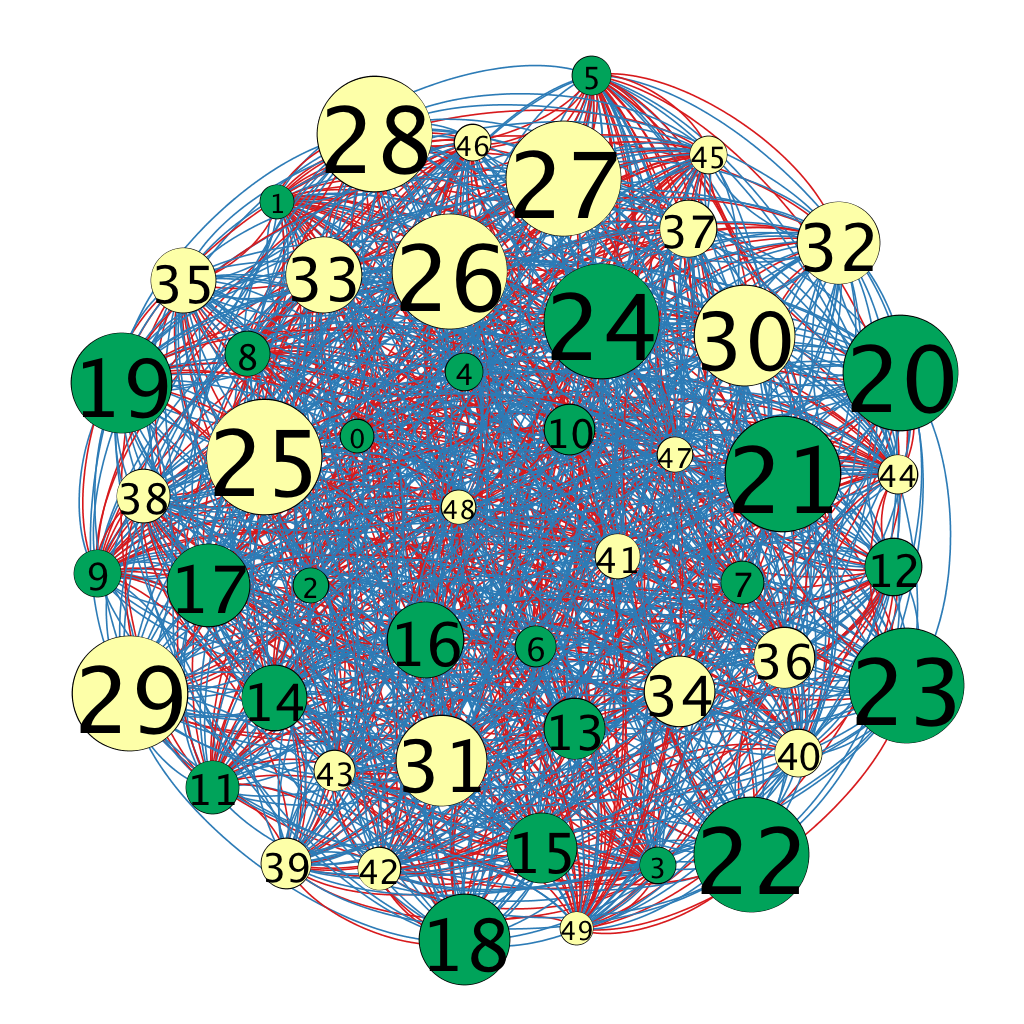
\includegraphics [scale = 0.3]{farmers_complete.png}
	\caption{\textit{Farmers network}. The nodes represent the farmers, numbered from 0 to 49, with their size being proportional to their signed degree; the edges represent the kind of relation two farmers have: blue for positive, red for negative. \textit{Gephi} identifies two modularity classes, green and yellow. Note that the nodes are split symmetrically at the center, and inside each class there are both friends and enemies.} 	\label{fig:50farmers}
\end{figure}
\begin{figure} [h]
	\centering
	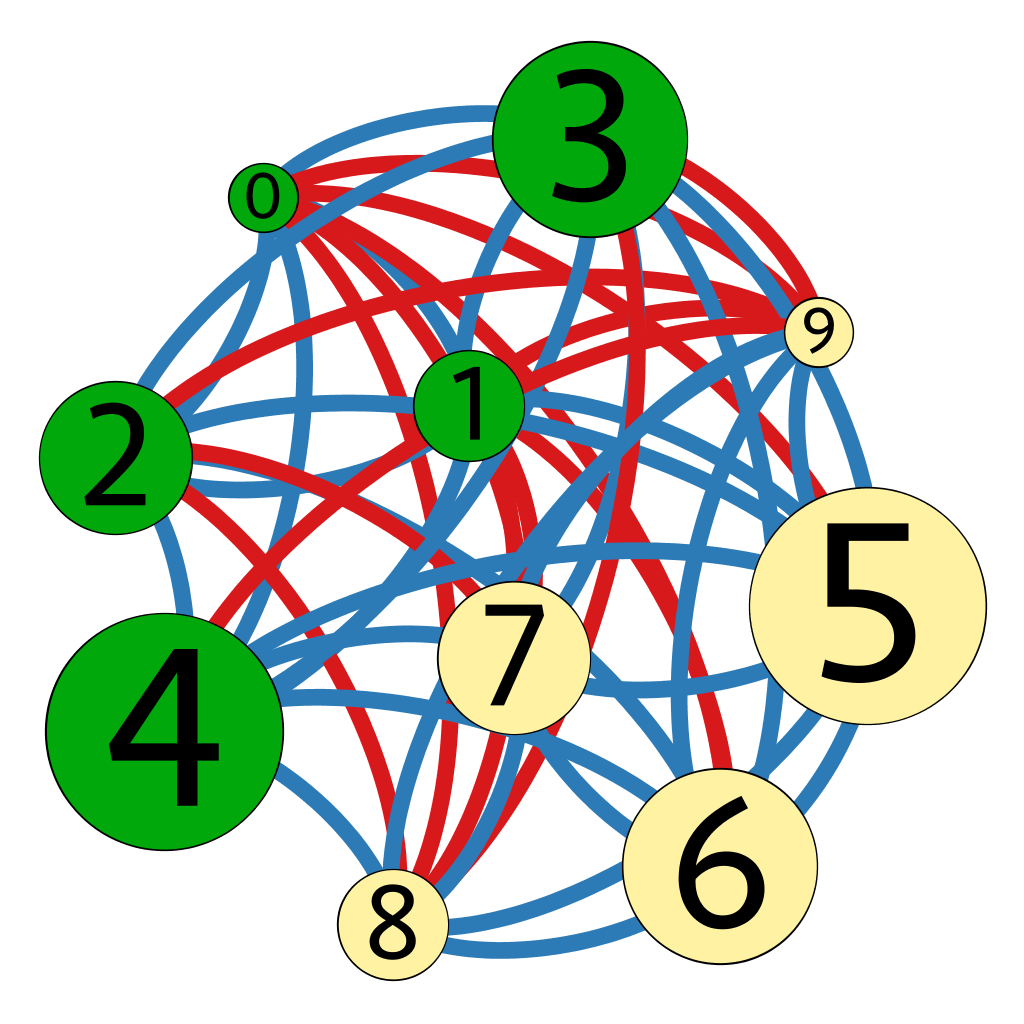
\includegraphics [scale = 0.3]{farmers_reduced.png}
	\caption{A smaller network (10 nodes, with \textit{friendship radius} of 4) for visualization purposes. It maintains the same structure as the complete one.}  \label{fig:10farmers}
\end{figure}

\newpage
Structural balance is an interesting and important property of complete signed networks that can be considered at two different but equivalent levels, local and global. Let us begin with the local point of view. We say that a signed network is \textbf{balanced} if all its triangles are balanced, i.e., if each of its triangles satisfies the \textbf{Structal Balance property}:
\bigskip

\textit{For every set of three nodes, if we consider the edges connecting them, either all three of these edges are labeled +, or else exactly one of them is labeled +}.
\bigskip


In our case the sign + represents friendship between farmers, the sign - represents antagonism.

Note that such property is a natural consequence of people tendency to avoid stressful situations in their social lives: indeed, a triangle with 2 sign + and only one sign -, represents the situation in which two people who do not get along with each other share a common friend. Although possible, this is a very unstable social situation: on the average, we expect that the common friend will be eventually able to change the situation, at least to some extent, so to have three mutual friends. By the same token, people tend to avoid situations in which there are three mutual enemies: history tells us that probably two of them will become allies.

It is easy to see in figure \ref{fig:50farmers} why our network does \textbf{not} satisfy the Structural Balance property. Let us denote by 1 the node representing the leftmost farmers, by 2 the node representing its neighbor, by 3 the node immediatly to the right of 2, ans so on. Let us now consider the triangle composed by nodes 1,2 and 21: being neighbors, 1 and 2 are friends. Moreover, also 2 and 21 are friends, since they live within 20 miles from each other. However, 1 and 21 are enemies, since they live at more than 20 miles from each other.

This simple example is enough to show that the network in not structurally balanced. However, let us see that such property does not hold also from a global point of view. The global counterpart of the Structural Balance property is the \textbf{Balance Theorem}.
\begin{thm}
	If a labeled complete graph is balanced, then either all pairs
	of nodes are friends, or else the nodes can be divided into two groups, X and Y ,
	such that every pair of nodes in X like each other, every pair of nodes in Y like
	each other, and everyone in X is the enemy of everyone in Y .
\end{thm}
Even from this other point of view it is easily seen that our graph is not balanced: first of all, it is immediate to see that not all nodes are friends. But it is also clear that they cannot be divided in two homogeneous groups of mutual friends which are all enemies of all members of the rival group. Consider again node 1 and 21: node 2 is friend of 1, hence it should belong to the set of 1's friends, say $X$. But it is also friend of 21, therefore it should also belong to the set of 21's friends, say $Y$. However, 1 and 21 are enemies, thus they must belong to two different groups. Once more, this example is enough to prove that the network is not balanced.\\
We understand that structural balance is a strong property to require from a real network. Therefore, out of curiosity, we check if a relaxed version of such property holds. Once more, we can regard this new concept from a local as well as from a global point of view. Let us start with the local one.\\
A complete signed graph is said to be \textbf{weakly balanced} if it sastifies the \textbf{Weakly Structural Balance property}:
\bigskip

\textit{There is no set of three nodes such that the edges among them consist of exactly two positive edges and one negative edge}.
\bigskip

In this relaxed version of the Balance property we allow the situation of three farmers which are mutual enemies: indeed, even though this situation could evolve into an alliance of two nodes, it is definitely less stressful, from a social point of view, than the one of two mutual enemies with a shared friend, which is still not admissible.\\
Unfortunately however, in our case this situation arises only in a portion of the triangles, such as in nodes 1, 21, 42, which all hate each other. Once more, the usual example of nodes 1, 2 and 21 is enough to show that our network is not weakly balanced. Out of curiosity, let us see the global counterpart of the weakly balance property.
\begin{thm}
	If a signed complete graph is weakly balanced, then its nodes can be divided into groups in such a way that every two nodes belonging to the same group are friends, and every two nodes belonging to different groups are enemies. 
\end{thm}
We see that, from a global point of view, the \textbf{Weak Balance theorem} allow an arbitrary number of homogeneous groups of friends. However, once more, nodes 1, 2 and 21 prove that the farmers' graph is not weakly balanced: indeed 2 should belong to the group of 1's friends and to the group of 21's friends as well, but 1 and 21 are enemies, thus they do not belong to the same group.

To sum things up, it seems that the way this network is structured is almost the \textit{opposite}, in some sense, to a structurally balanced network, since we will never be able to split the graph in subgraphs all friends with each other.
\newpage

\section*{Exercise 21.3}
In this exercise we are trying to design efficient measures to control the outbreak of an epidemic in its early stages within a livestock  population. Two different actions are possible: trying to control the extent to which the
animals come in contact with each other, and introducing higher levels of sanitization to reduce the probability that one animal passes the disease to another. Clearly these measures cost money, and we have a budget of 2 million dollars.

We estimate that spending $x$ dollars to control the extent to which animals come in contact with each other will change such number in
\begin{equation*}
40-\frac{x}{200,000}
\end{equation*}
At the same time, we estimate that spending $y$ dollars to introduce sanitization measures to reduce the probability of transmission will change such probability into
\begin{equation*}
0.04-\frac{y}{100,000,000}
\end{equation*}
Agricultural officials are planning to spend one million on each of these two kinds of the measures. However, we are going to argue that there are better ways to spend such money.

First of all, let us pose the problem into a coherent framerwork: we model the livestocks' population as a tree, and the epidemic as a \textbf{branching process} over it. Each edge from a node in level i--th to another node in level (i+1)--th respresents the fact that two animals come in contact with each other.
\begin{figure} [h]
	\centering
	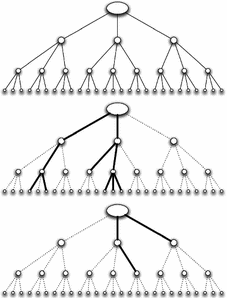
\includegraphics [width=7cm,height=7cm,keepaspectratio]{Branching_giusto.png}
	\label{Bra}
	\caption{Example of a branching process describing an epidemics.}
\end{figure}


 Let us now denote by $q_n$ the probability that the epidemic survives for at least $n$ waves — in other words, that some individual in the n--th level of the tree becomes infected. Let $q^*$ be the limit of $q_n$ as $n \rightarrow \infty$. We know that the surviving of an epidemics critically depends on its \textbf{basic reproductive number} $R_0 = kp$, where $k$ is the number of other individuals an infected individual meets and $p$ represents the probability of transmission of the disease. It is possible to prove that 
\bigskip 

\textit{If $R_0<1$ then $q^* = 0$. If $R_0>1$ then $q^*>0$.}
\bigskip

Clearly, in our case,
\begin{equation} \label{R}
R_0 = \left(40-\frac{x}{200,000}\right)\left(0.04-\frac{y}{100,000,000}\right)
\end{equation}
Therefore, any measure to control the epidemic must be such that $\eqref{R}$ is less than $1$. First of all, let us check if the strategy proposed by the agricultural officials is at least sufficient to stop the disease, in the long term: with $x = 1,000,000$ and $y = 1,000,000$
\begin{equation*}
R_0 = 1.05
\end{equation*}
which shows that the proposal of the agricultural officers is not even able to stop the epidemic. Out of curiosity, let us see what happens if we devote all the resources to only one measure; if we spend two millions for controlling the number of individuals that come in contact with each other - in other words to minimize $k$ - we get $R_0 = 1.2$. Instead, if we spend two millions for reducing the probability of contagious - in other words to minimize $p$ - we get $R_0 = 0.8$. Hence the latter strategy, i.e., devote all the resources to improve hygiene, is a viable strategy, better than the one originally proposed. 
We want now to understand which is the best way to deploy our resources: to do so, we have to find $x$ and $y$ for which $R_0$ is minimized. We have the following set of constraints
\begin{equation*}
\begin{cases}
x\geq 0
\\ x \leq 2*10^6
\\ y = 2*10^6-x
\end{cases}
\end{equation*}
\begin{figure} [h]
	\centering
	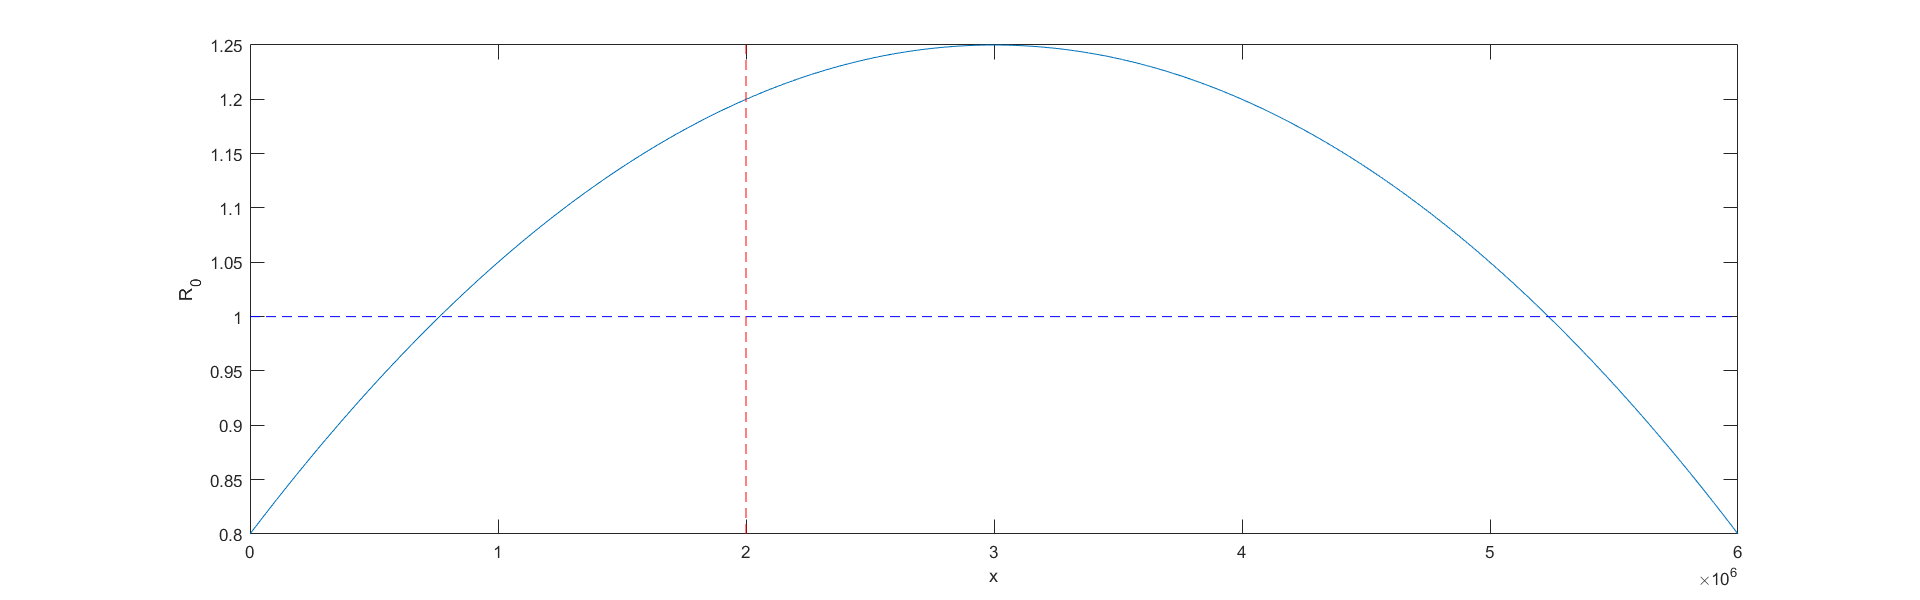
\includegraphics [width=12cm,height=17cm,keepaspectratio]{parabola.png}
	\label{Par}
	\caption{$R_0$ as a function of $x$.}
\end{figure}


From the plot we see that the minimum for $R_0$ is indeed reached at $x = 0$, that corresponds to devoting all two million dollars for reducing the probability of contagious.

However, since our goal is just to mantain $R_0<1$, we may also be satisfied with, for example, $R_0 = 0.95$. This can be achieved  by taking $x = 0$ and $y = 1,625,000$: therefore by spending only $1,625,000$ millions, hence saving $375,000$ dollars, we are still able to stop the epidemics on the long run.
\end{document}